\message{ !name(relatorio.tex)}\documentclass{article}
\author{Pedro de Carvalho Braga Ilidio Silva}
\title{Projeto 4 — Movimento realístico}
\date{19 de maio de 2017}

\usepackage[utf8]{inputenc}
\usepackage{listings}
\usepackage{graphicx}
\usepackage{listings}

\begin{document}

\message{ !name(relatorio.tex) !offset(-3) }

\maketitle
\section{Introdução}

\section{Efeito resistivo do ar em bicicletas}

Partir-se-á da seguinte equação, que se trata de uma aproximação numérica para a velocidade \(v\) de uma massa pontual em movimento retilíneo (bicicleta), obtida por meio do Método de Euler.

\begin{equation}
  \label{eq:vel}
  v_{i+1} = v_i + \frac{P}{mv_i} \Delta t -\frac{\rho Av^2_i}{2m} \Delta t
\end{equation}

É facilmente perceptível pela equação \ref{eq:vel}, a inviabilidade de se aplicar este método a movimentos posteriores a instantes de repouso, em que a velocidade é nula, pois deparar-se-ia com divisão por zero no segundo termo e não seria possível dar continuidade aos procedimetos recursivos.\par
Foram definidas os seguintes termos como constantes:

\begin{list}{}{}
\item Massa: \(m = 70 kg\)
\item Potência: \(P = 400 W\)
\item Duração do movimento, máximo instante considerado: \(t_{max}=300 s\)
\item Intervalo entre os instantes de tempo considerados: \(\Delta t = 0.1s\)
\item Velocidade inicial: \(v_0 = 4 m/s\)
\end{list}

A partir dos quais foi elaborado um programa em Fortran90 para estimar a velocidade da bicicleta nos instantes determinados pelos parâmetros.

\begin{lstlisting}
    DO I = 1, INT(TMAX/DT)
       RES(I, COL) = V
       V = V + P/(M*V)*DELTAT - (RHO*A*V**2)/(2*M) * DELTAT
    END DO
\end{lstlisting}

Os valores foram então coletados e graficados.

\begin{figure}[h]
  \centering
  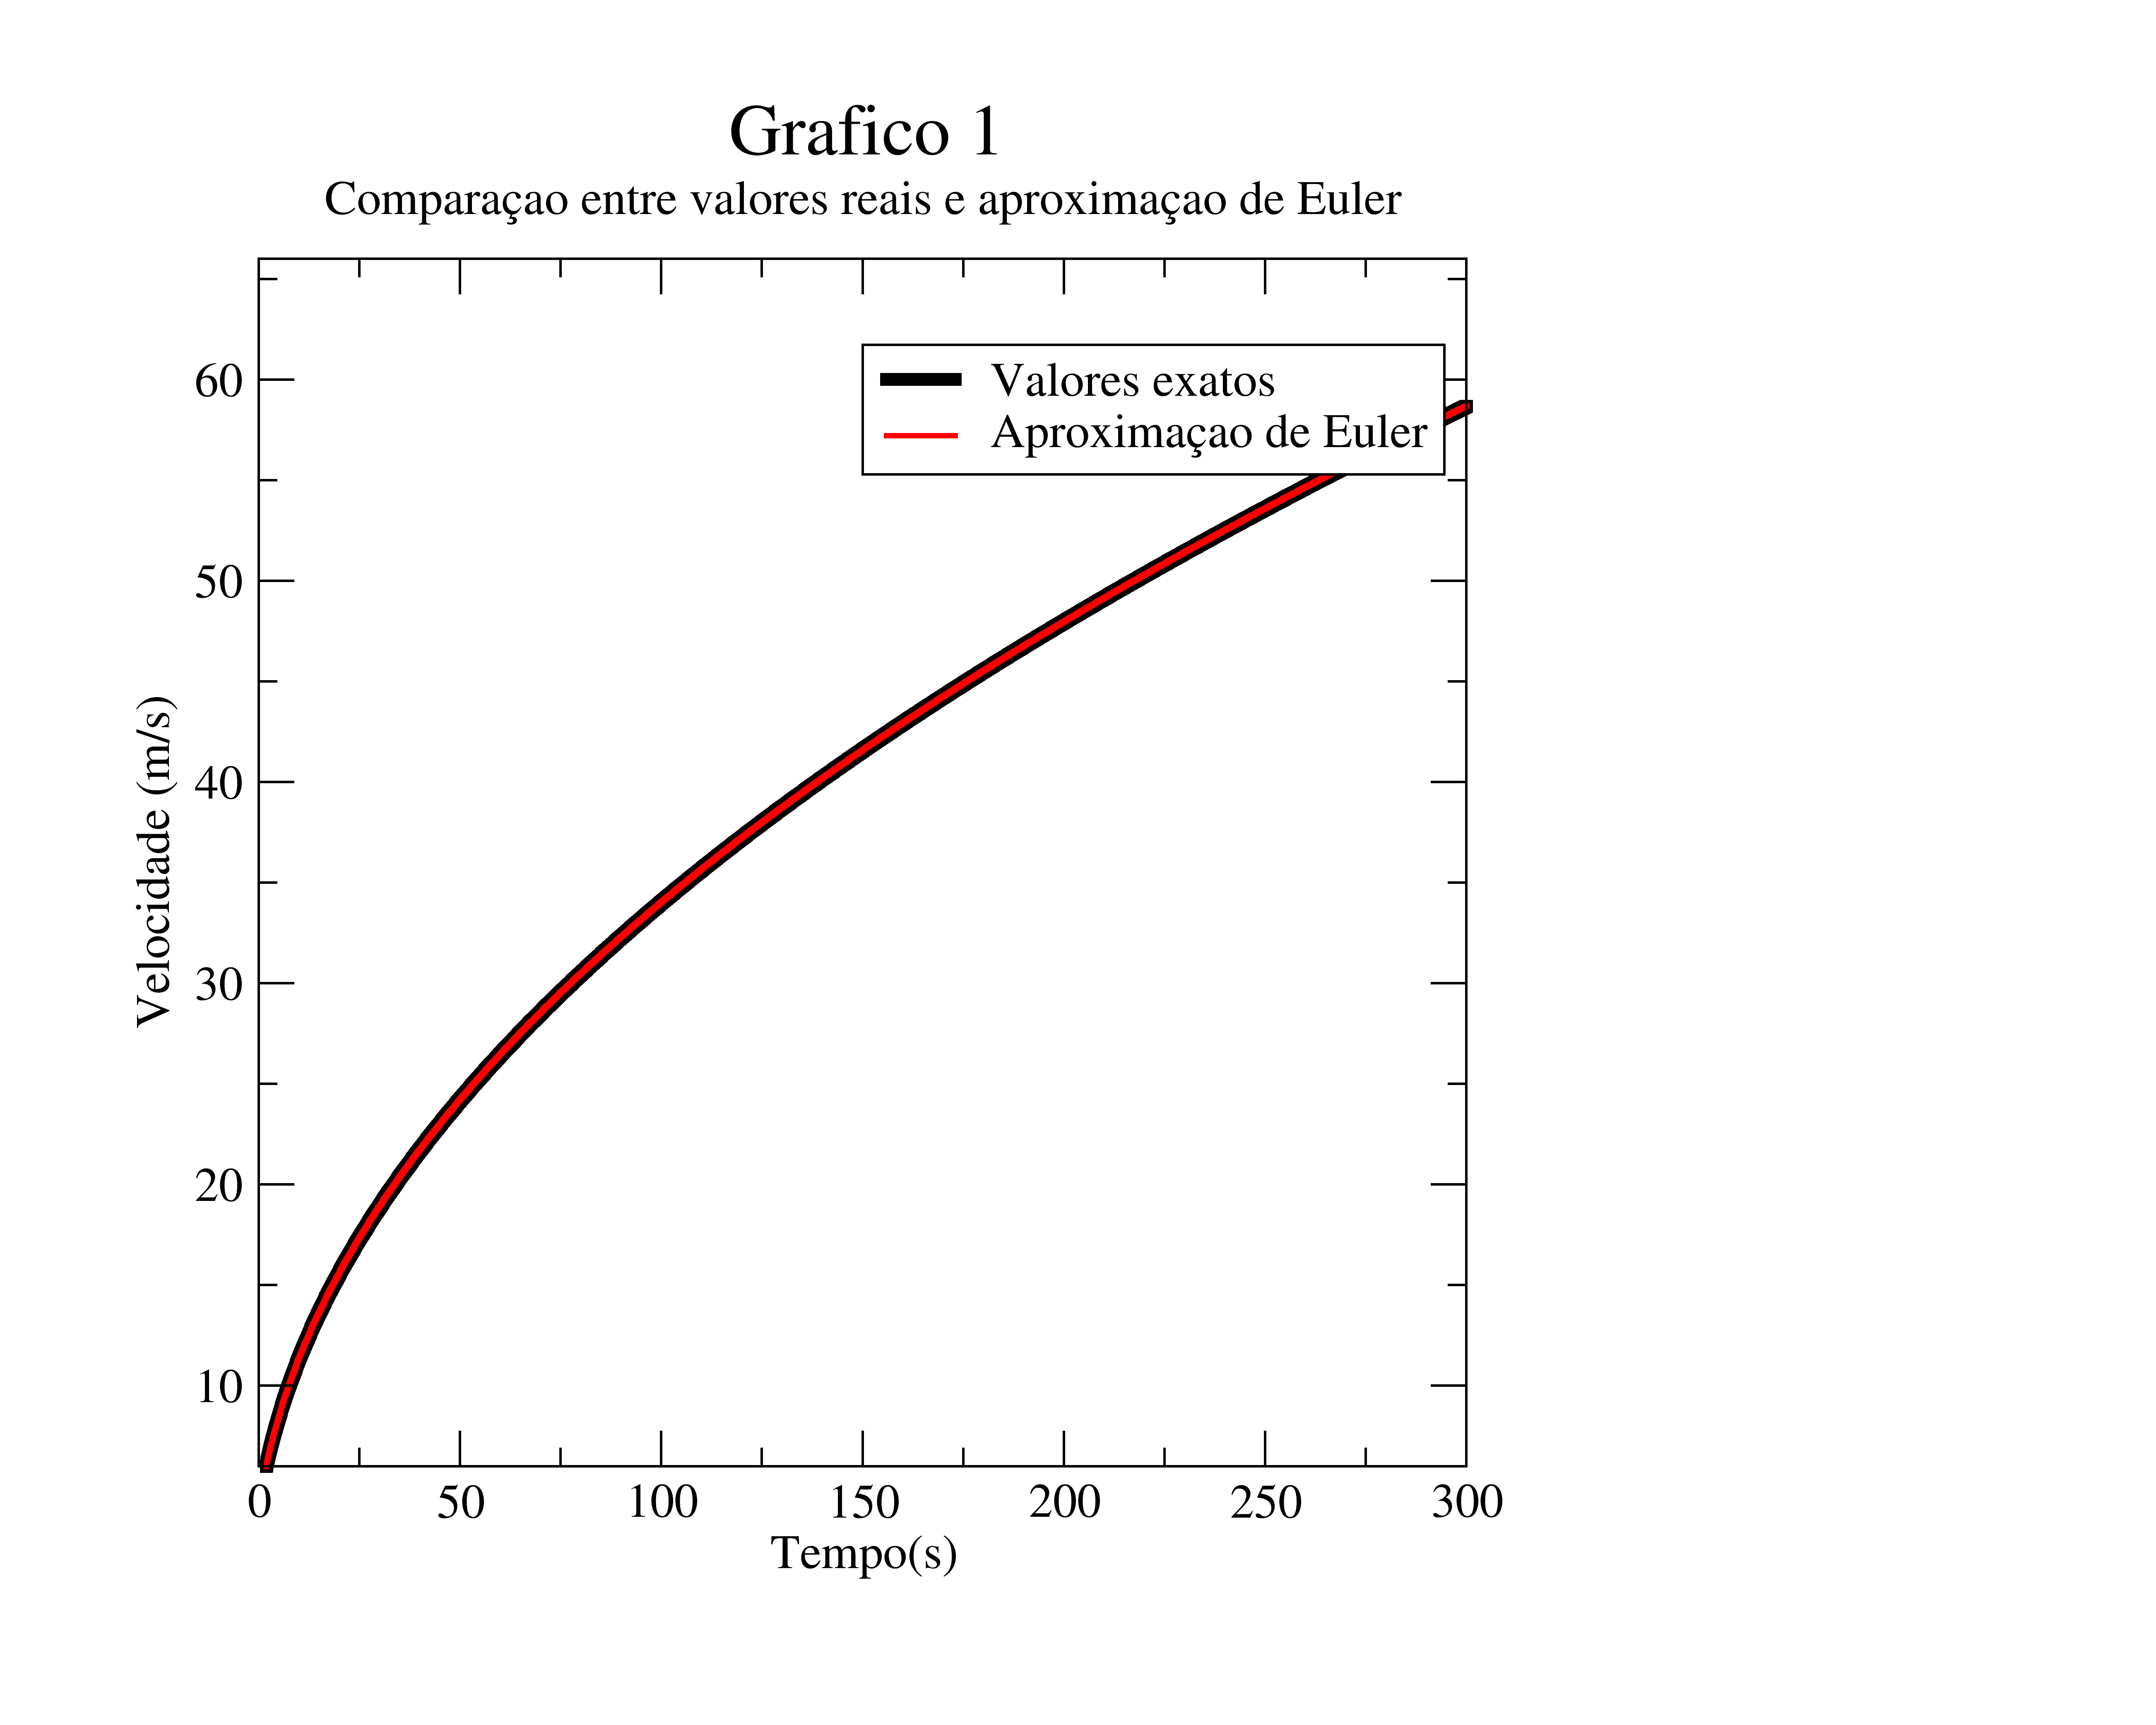
\includegraphics[width=\textwidth]{graf1}
\end{figure}


\end{document}

\message{ !name(relatorio.tex) !offset(-57) }
